\chapter{Results \& Snapshots}
\thispagestyle{special}
\centerline{
\includegraphics[scale=0.20]{landing.png}}
\centering{Fig.5.1. Landing page}

\justifying{
 Figure 5.1 describes the landing page, sometimes known as a "lead capture page", "single property page", "static page", "squeeze page" or a "destination page", is a single web page that appears in response to clicking on a search engine optimized search result, marketing promotion, marketing email or an online advertisement.[1] The landing page will usually display directed sales copy that is a logical extension of the advertisement, search result or link. Landing pages are used for lead generation. The actions that a visitor takes on a landing page are what determine an advertiser's conversion rate. A landing page may be part of a micro site or a single page within an organization's main website.It is used to display the landing page of the website.}


\thispagestyle{special}
\centerline{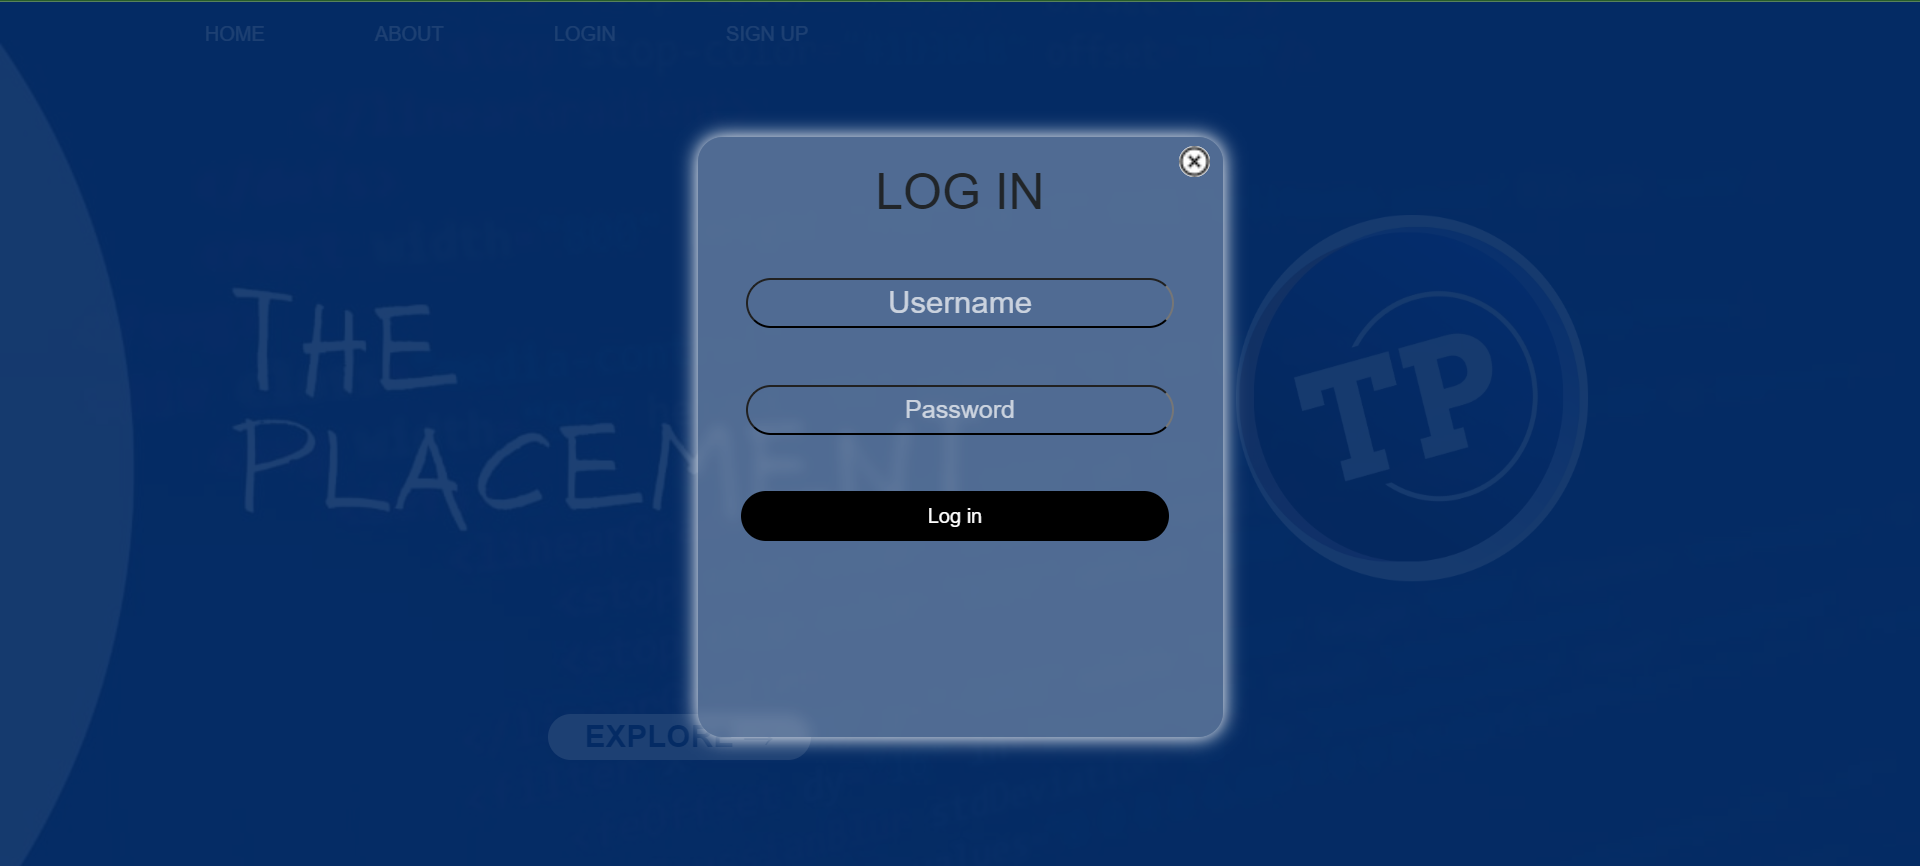
\includegraphics[scale=0.30]{login.png}}
\centering{Fig.5.2. Login page}

\justifying{
 Figure 5.2 describes the login page, A login page specifies the login URL in a web application that users must pass through to get to the authenticated URL at the heart of the application. Authenticated URLs are URLs that become accessible to users only after they successfully log in to the login URL.}
 

\thispagestyle{special}
\hspace
\centerline {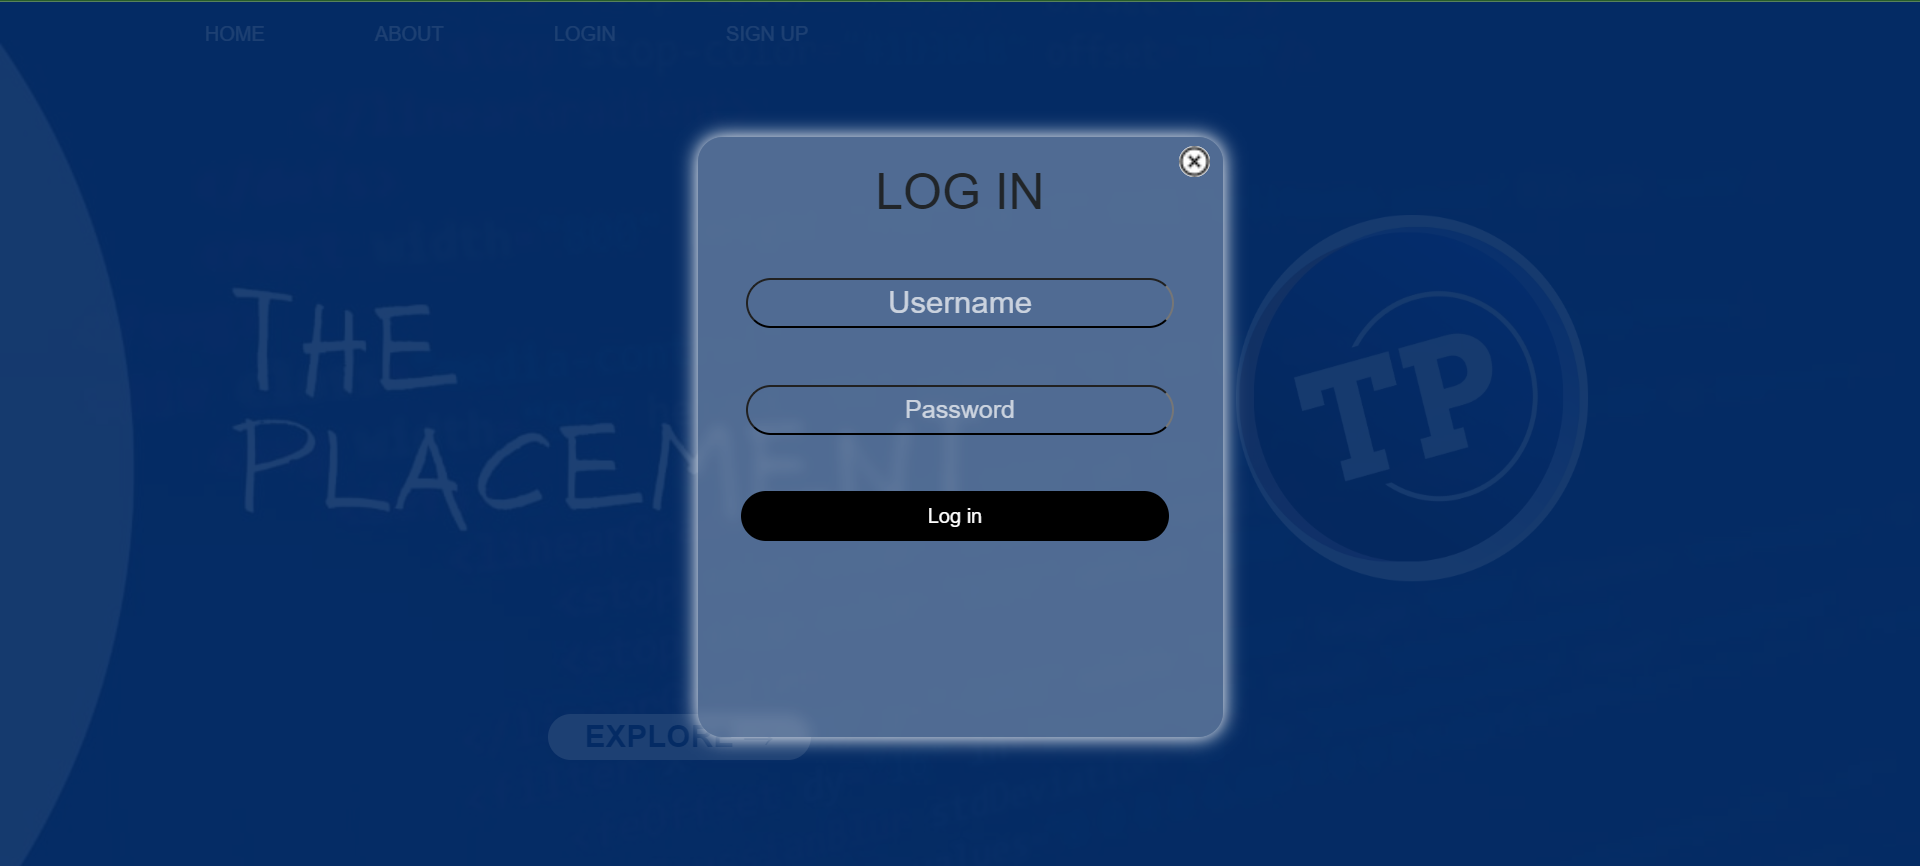
\includegraphics[scale = .30]{login.png}}
\centering{Fig.5.3. Another page}

\justifying{
 Figure 5.3 describes the login page, A login page specifies the login URL in a web application that users must pass through to get to the authenticated URL at the heart of the application. Authenticated URLs are URLs that become accessible to users only after they successfully log in to the login URL.}
 
